% ============================================================
%  INFORME DE PRÁCTICA PROFESIONAL SUPERVISADA
%  Reparación y Rediseño de Sintetizador de Frecuencias Banda Ku
% ============================================================
\documentclass[12pt, a4paper]{article}

% --- Paquetes ---
\usepackage[spanish, es-tabla]{babel}
\usepackage[utf8]{inputenc}
\usepackage[T1]{fontenc}
\usepackage{geometry}
\geometry{top=2.5cm, bottom=2.5cm, left=3cm, right=2.5cm}

\usepackage{graphicx}
\usepackage{float}
\usepackage{booktabs}
\usepackage{array}
\usepackage{amsmath}
\usepackage{amssymb}
\usepackage{hyperref}
\usepackage{fancyhdr}
\usepackage{titlesec}
\usepackage{setspace}
\usepackage{parskip}
\usepackage{caption}
\usepackage{subcaption}
\usepackage{xcolor}
\usepackage{tcolorbox}
\usepackage{enumitem}
\usepackage{listings}
\usepackage{microtype}
\usepackage{lmodern}
\usepackage{pdfpages}

% --- Color institucional ---
\definecolor{azulUNT}{RGB}{0, 51, 102}
\definecolor{grisClaro}{RGB}{230, 230, 230}
% --- Encabezado y pie de página ---
\pagestyle{fancy}
\fancyhf{}
\fancyhead[L]{\small\textcolor{azulUNT}{PPS – Sintetizador de Frecuencias Banda Ku}}
\fancyhead[R]{\small\textcolor{azulUNT}{UNT – FCEyT}}
\fancyfoot[C]{\thepage}
\renewcommand{\headrulewidth}{0.4pt}

% --- Formato de títulos ---
\titleformat{\section}
{\large\bfseries\color{azulUNT}}
{\thesection.}{0.5em}{}[\titlerule]

\titleformat{\subsection}
{\normalsize\bfseries\color{azulUNT}}
{\thesubsection}{0.5em}{}

\titleformat{\subsubsection}
{\normalsize\itshape\bfseries}
{\thesubsubsection}{0.5em}{}

% --- Listings (código) ---
\lstset{
	basicstyle=\ttfamily\small,
	keywordstyle=\color{azulUNT}\bfseries,
	commentstyle=\color{gray}\itshape,
	stringstyle=\color{red!60!black},
	numbers=left,
	numberstyle=\tiny\color{gray},
	frame=single,
	breaklines=true,
	captionpos=b,
	language=C++
}

% --- Interlineado ---
\setstretch{1.15}

% ============================================================
\begin{document}
	
	% ============================================================
	%  PORTADA
	% ============================================================
	\thispagestyle{empty}
	\begin{titlepage}
		\centering
		\vspace*{0.5cm}
		
		{\Large \textbf{Universidad Nacional de Tucumán}}\\[0.3cm]
		{\large Facultad de Ciencias Exactas y Tecnología}\\[0.2cm]
		{\large Carrera: Ingeniería en Electrónica}\\[2cm]
		
		\noindent\rule{\textwidth}{1.5pt}\\[0.4cm]
		{\LARGE \textbf{Reparación y Rediseño de un\\[0.2cm]
				Sintetizador de Frecuencias en Banda Ku}}\\[0.3cm]
		\noindent\rule{\textwidth}{1.5pt}\\[1.5cm]
		
		{\large \textbf{Informe de Práctica Profesional Supervisada}}\\[2cm]
		
		\begin{minipage}[t]{0.48\textwidth}
			\raggedright
			\textbf{Autor:}\\
			Alexis Vale
			Jesús Avila
		\end{minipage}
		\hfill
		\begin{minipage}[t]{0.48\textwidth}
			\raggedleft
			\textbf{Directores:}\\
			Fernando Miranda Bonomi\\
			Juan Ise
		\end{minipage}\\[2cm]
		
		\textbf{Lugar de realización:}\\
		Laboratorio de Telecomunicaciones – FaCET – UNT\\[1cm]
		
		\textbf{Período:} 2025–2026\\[2cm]
		
		\vfill
		{\small Tucumán, Argentina}
	\end{titlepage}
	
	% ============================================================
	%  RESUMEN
	% ============================================================
	\newpage
	\thispagestyle{plain}
	\section*{Resumen}
	\addcontentsline{toc}{section}{Resumen}
	
	El presente informe describe el proceso de recuperación y rediseño integral de un sintetizador de
	frecuencias para microondas diseñado para operar en la banda Ku (10{,}6~GHz a 11{,}8~GHz),
	originalmente desarrollado en 2009 y recibido en estado no funcional. El trabajo abarcó el diagnóstico
	del hardware heredado, la identificación de fallas críticas en el oscilador controlado por tensión (VCO),
	el reemplazo de componentes dañados y, finalmente, el rediseño completo del circuito impreso (PCB)
	ante la degradación acumulada por múltiples intervenciones previas.
	
	Como parte del rediseño, el controlador original (microcontrolador PIC) fue reemplazado por una
	plataforma ESP32, incorporando comunicación Bluetooth e interfaz de usuario. La validación funcional
	se realizó en el banco de microondas del Laboratorio de Telecomunicaciones, confirmando el
	enclavamiento del lazo PLL con un error relativo menor al 0{,}15\% a lo largo de toda la banda operativa.
	
	\bigskip
	\noindent\textbf{Palabras clave:} sintetizador de frecuencias, banda Ku, PLL, VCO, ESP32, microondas, rediseño PCB.
	
	% ============================================================
	%  ÍNDICE
	% ============================================================
	\newpage
	\tableofcontents
	\newpage
	
	% ============================================================
	%  1. INTRODUCCIÓN
	% ============================================================
	\section{Introducción}
	
	\subsection{Contexto del sistema}
	
	El equipo objeto del presente trabajo es un sintetizador de frecuencias para microondas diseñado para
	operar en la banda Ku. Fue desarrollado originalmente en el año 2009 y basa su funcionamiento en un
	lazo de seguimiento de fase (\textit{Phase-Locked Loop}, PLL), compuesto por un oscilador controlado
	por tensión (VCO HMC534LP5) y un sintetizador de frecuencias integrado (SP\,5769), controlado
	mediante bus I2C.
	
	El equipo fue recibido en estado completamente no funcional: presentaba ausencia total de la etapa de
	alimentación y daños severos en el módulo de control e interfaz (la placa donde residía el
	microcontrolador encargado de la selección de frecuencia). Adicionalmente, la inspección de la placa
	principal de RF reveló indicios de intentos de reparación previos no documentados: pistas de cobre
	recubiertas con estaño, cortes en el ruteo original y puentes improvisados para restituir continuidad
	eléctrica. Este nivel de deterioro comprometía severamente la integridad de las señales de alta frecuencia.
	
	\subsection{Aplicación}
	
	El propósito del proyecto es el reacondicionamiento integral del equipo para incorporarlo como
	instrumento de trabajo en el Laboratorio de Telecomunicaciones de la Facultad de Ciencias Exactas y
	Tecnología de la Universidad Nacional de Tucumán. El sistema restaurado tendrá un fin estrictamente
	educativo y didáctico, permitiendo a los estudiantes de futuras cursadas y proyectos de investigación
	realizar prácticas reales con señales de microondas, facilitando la comprensión práctica de conceptos
	avanzados de RF y lazos de seguimiento de fase (PLL).
	
	\subsection{Objetivo del trabajo}
	
	El objetivo principal es recuperar la operatividad total del sintetizador de microondas. Debido a las fallas
	acumuladas por deterioro del hardware, la obsolescencia técnica de su implementación física y los
	intentos de reparación previos infructuosos, el trabajo no se limita a una reparación puntual: requiere
	un \textbf{rediseño integral de la PCB} para garantizar la estabilidad del sistema, minimizar pérdidas y
	asegurar su funcionamiento a largo plazo.
	
	\subsection{Alcance}
	
	Para cumplir con los objetivos planteados, el proyecto abarca las siguientes etapas:
	
	\begin{enumerate}[leftmargin=*, label=\textbf{\arabic*.}]
		\item \textbf{Diagnóstico:} Relevamiento detallado del estado actual de los componentes heredados y
		análisis crítico del circuito original.
		\item \textbf{Reparación inicial:} Pruebas de supervivencia de los componentes críticos (VCO y
		sintetizador) y montaje de una alimentación provisoria.
		\item \textbf{Rediseño de PCB:} Migración del diseño esquemático y desarrollo de una nueva placa de
		circuito impreso (mediante KiCad y AWR), solucionando los problemas de ruteo e integridad de
		señal de la versión anterior.
		\item \textbf{Validación funcional:} Mediciones en banco de microondas para asegurar el enclavamiento
		en frecuencia y la potencia de salida esperada.
	\end{enumerate}
	
	% ============================================================
	%  2. DESCRIPCIÓN DEL SISTEMA ORIGINAL
	% ============================================================
	\section{Descripción del sistema original}
	
	\subsection{Arquitectura general}
	
	El sintetizador opera bajo el principio de síntesis directa mediante lazo de seguimiento de fase (PLL).
	Los componentes principales del sistema heredado son:
	
	\begin{itemize}[leftmargin=*]
		\item \textbf{Sintetizador/PLL:} SP\,5769 (Phillips/NXP), controlado por bus I2C.
		\item \textbf{Oscilador controlado por tensión (VCO):} HMC534LP5 (Analog Devices/Hittite),
		encapsulado QFN de 5$\times$5\,mm.
		\item \textbf{Controlador original:} Microcontrolador PIC16F873A, encargado de la programación de
		registros del PLL.
		\item \textbf{Transistor externo:} BCW\,31 en configuración amplificador inversor, para adaptar la
		tensión de sintonía (\textit{Vtune}) requerida por el VCO (0–13\,V) desde la salida de 5\,V del
		sintetizador.
	\end{itemize}
	
\begin{figure}[H]
	\centering
	\fcolorbox{azulUNT}{white}{
		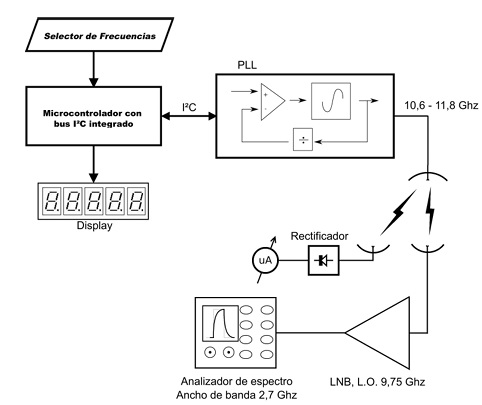
\includegraphics[width=0.85\textwidth]{img/DiagramaBloquesSistemaOriginal}
	}
	\caption{Diagrama en bloques del sistema original.}
	\label{fig:bloques_original}
\end{figure}
	
	\subsection{Funcionamiento}
	
	\subsubsection{Generación de frecuencia}
	El VCO genera una señal de RF cuya frecuencia depende de la tensión aplicada en su pin de sintonía
	(\textit{Vtune}). El sintetizador SP\,5769 implementa el lazo PLL: divide la señal de salida del VCO
	mediante divisores programables, la compara con una referencia interna de cristal y genera una señal
	de error (bomba de carga) que, a través del amplificador externo con el BCW\,31, ajusta \textit{Vtune}
	hasta que la frecuencia de salida coincide con la programada.
	
	\subsubsection{Control e interfaz}
	El PIC16F873A (en el diseño original) programa los registros internos del SP\,5769 vía bus I2C,
	estableciendo los valores de los divisores de frecuencia que determinan la frecuencia de síntesis.
	
	\subsubsection{Rango de salida RF}
	El sistema está diseñado para operar en el rango de \textbf{10{,}6\,GHz a 11{,}8\,GHz}, cubriendo la
	banda Ku de interés.
	
	\subsection{Limitaciones detectadas}
	
	\begin{itemize}[leftmargin=*]
		\item \textbf{Dependencia del SP\,5769:} Al tratarse de un componente específico ya presente en la
		placa original, su disponibilidad en el mercado actual es limitada. Durante el proyecto, el
		SP\,5769 original resultó dañado, requiriéndose la adquisición de uno nuevo con distinto
		encapsulado, lo que obligó a adaptar la huella en la PCB rediseñada.
		\item \textbf{Dificultad de mantenimiento:} Las múltiples reparaciones sucesivas sobre la placa
		original fueron degradando progresivamente las soldaduras y la integridad física de los
		componentes, haciendo inevitables el rediseño completo de la PCB y el reemplazo con
		componentes nuevos.
		\item \textbf{Encapsulado QFN del VCO:} El HMC534LP5 carece de pines expuestos tradicionales,
		concentrando su disipación térmica en la almohadilla central inferior. Esto hace que su soldadura
		y reemplazo sean técnicamente exigentes y requieran equipamiento especializado.
		\item \textbf{El microcontrolador usado es muy antiguo} Se decidipo cambiar por un ESP32 por su menor precio, ensamblado comodo en pcb, posibilidad de programar en C/Arduino y su conexión Bluetooth.
	\end{itemize}
	
	% ============================================================
	%  3. DIAGNÓSTICO Y FALLA
	% ============================================================
	\section{Diagnóstico y falla}
	
	\subsection{Análisis inicial e implementación de hardware de prueba}
	
	El proceso de diagnóstico comenzó con el estudio de las hojas de datos (\textit{datasheets}) de los
	componentes críticos: el sintetizador SP\,5769 y el VCO HMC534LP5. Se determinaron los niveles de
	tensión necesarios para la operación y se realizó una inspección visual del conexionado.
	
	Dado que el sistema se recibió sin su etapa de alimentación original, fue necesario utilizar hardware
	auxiliar:
	
	\begin{itemize}[leftmargin=*]
		\item \textbf{Alimentación de 12\,V:} Se diseñó y fabricó una fuente regulable de 12\,V utilizando el método de transferencia térmica (planchado) para la creación de la placa de circuito impreso (PCB).
		\item \textbf{Alimentación de 5\,V:} Para la lógica de control, se utilizó directamente la salida regulada de 5\,V provista por la placa de desarrollo ESP32.
		\item \textbf{Interfaz de conexión (Shield ESP32):} Se fabricó una placa adaptadora (tipo \textit{poncho} o \textit{shield}), también mediante el método de transferencia térmica, para interconectar de manera segura la ESP32 con la placa de RF heredada.
	\end{itemize}

	\begin{figure}[H]
		\centering
		\begin{subfigure}{0.45\textwidth}
			\centering
			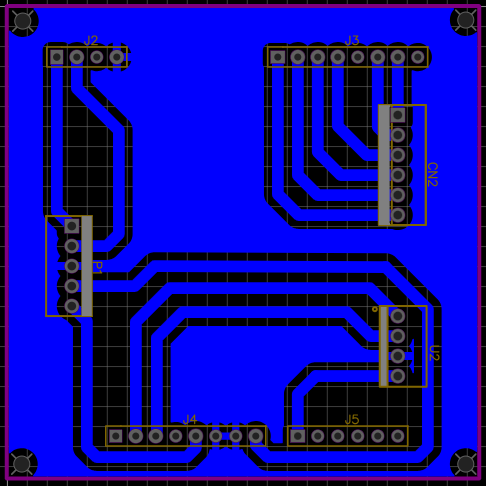
\includegraphics[width=\linewidth]{images/image32.png}
			\caption{Vista superior}
		\end{subfigure}
		\hfill
		\begin{subfigure}{0.45\textwidth}
			\centering
			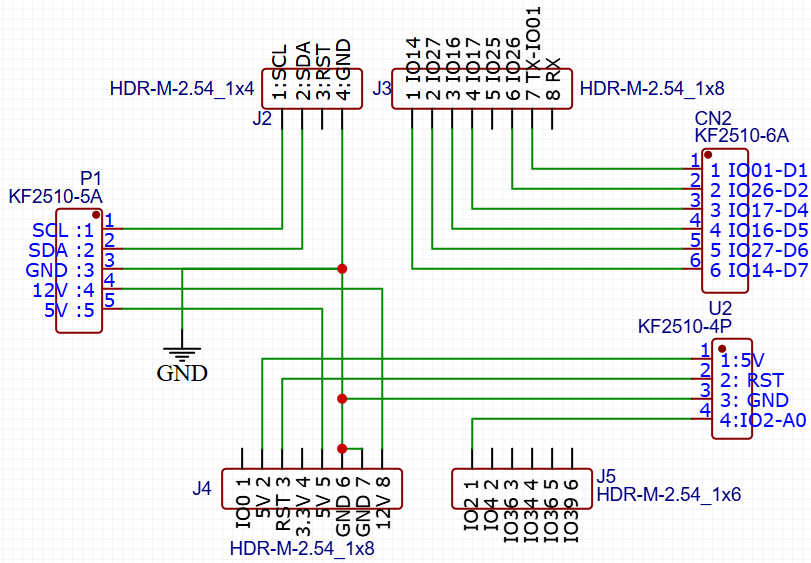
\includegraphics[width=\linewidth]{images/image34.png}
			\caption{Vista inferior}
		\end{subfigure}
		\caption{Shield ESP32 implementado provisionalmente.}
		\label{fig:shield_esp32}
	\end{figure}
	
	\subsection{Desarrollo de firmware}
	
	El código fuente original (desarrollado para PIC16F873A) resultó de difícil comprensión y adaptación.
	Se decidió descartar el firmware existente y desarrollar uno nuevo desde cero sobre la plataforma
	ESP32, basándose estrictamente en los registros y diagramas de tiempos especificados en la hoja de
	datos del SP\,5769. El repositorio del nuevo firmware se encuentra disponible en:
	\url{https://github.com/gsuckz/pll} 
	
	Tras múltiples pruebas y ajustes de sincronización, se logró establecer comunicación exitosa a través
	del bus I2C entre la ESP32 y el SP\,5769, confirmando que la lógica digital del sintetizador se
	encontraba operativa. Se detectó y corrigió además un error en los valores asignados a uno de los
	divisores programables.
	
	\subsection{Falla principal: daño en el VCO}
	
	\subsubsection{Síntomas observados}
	El día 29 de agosto de 2024 se realizaron las primeras pruebas formales sobre el banco de microondas
	(ver Informe de Actividades de Laboratorio adjunto en Anexo). Los síntomas observados fueron:
	
	\begin{itemize}[leftmargin=*]
		\item Ausencia total de potencia de salida de RF, confirmada con sensor rectificador con medidor
		analógico y con analizador de RF digital.
		\item El PLL no lograba el enclavamiento (\textit{no lock}) a pesar de que el SP\,5769 respondía
		correctamente a los comandos I2C y permitía fijar la frecuencia programada.
		\item Al analizar el lazo cerrado, el sintetizador intentaba ajustar \textit{Vtune} para corregir la
		frecuencia, pero no recibía señal de realimentación (\textit{feedback}) por parte del VCO.
	\end{itemize}
	
	\subsubsection{Diagnóstico conclusivo}
	Descartados errores en el código (corregidos previamente), en el conexionado y en los niveles de
	alimentación, se concluyó que el VCO HMC534LP5 estaba \textbf{dañado irreversiblemente de forma
		previa} a la recepción del equipo.
	
	\subsection{Reemplazo del VCO (encapsulado QFN)}
	
	La confirmación de la falla del VCO obligó a su reemplazo, lo cual representó un desafío técnico
	significativo debido al encapsulado QFN de 5$\times$5\,mm: carece de pines expuestos y concentra su
	disipación térmica en la almohadilla central inferior. Se aplicaron técnicas de soldadura térmica
	adecuadas para este tipo de empaquetado, logrando extraer el componente dañado y montar
	exitosamente la unidad de reemplazo. Para este procedimiento fue necesario recurrir a la asistencia
	técnica de \textbf{DIGICOM}, dado que el proceso requería equipamiento especializado.
	
	\subsection{Problemas de alimentación y reestructuración}
	
	Tras la instalación del nuevo VCO, el sistema mostraba actividad pero no lograba enclavarse. Se
	detectó que el regulador interno de la ESP32 no poseía la capacidad de corriente suficiente para
	alimentar simultáneamente la lógica digital, el sintetizador y el VCO. La caída en la línea de 5\,V
	(por debajo de 4{,}5\,V) desestabilizaba por completo el lazo de sintonía.
	
	Se reestructuró la arquitectura de alimentación:
	
	\begin{itemize}[leftmargin=*]
		\item \textbf{Separación de fuentes:} Se incorporó una fuente conmutada (\textit{switching}) dedicada
		exclusivamente a proveer los 5\,V robustos que demandan los componentes de RF (VCO y
		sintetizador), con masa común a la etapa de control digital (ESP32).
		\item \textbf{Gestión de Vtune:} Se verificó el correcto funcionamiento del amplificador inversor
		discreto (BCW\,31), alimentado por la línea de 12\,V y comandado por la salida \textit{Drive}
		del SP\,5769, encargado de proveer la amplitud de tensión necesaria (0–13\,V) para el control
		del VCO.
	\end{itemize}
	
	Adicionalmente, se identificó el ventilador (\textit{cooler}) acoplado al disipador térmico del VCO
	como posible fuente de ruido. De manera preventiva, se diseñó e implementó un filtro activo pasa-bajos
	compuesto por un transistor NPN 2N2222 en configuración emisor seguidor, una resistencia de base de
	33\,k$\Omega$ y un capacitor de 10\,\textmu F, logrando desacoplar la línea de alimentación de RF
	de las posibles interferencias.
	
	\subsection{Falla y obsolescencia definitiva del hardware heredado}
	
	Tras múltiples intervenciones sobre la PCB original, la placa acumuló un deterioro físico significativo.
	El reemplazo del VCO original, que se encontraba dañado, implicó varias operaciones de desoldado y
	resoldado que degradaron las pistas y almohadillas. Durante estas tareas, un segundo VCO también
	resultó dañado debido a un error de manipulación, lo que agravó el estado general del circuito impreso.
	
	Como consecuencia de estas intervenciones sucesivas, la integridad mecánica y eléctrica de la PCB se
	vio comprometida, volviendo poco confiable su reutilización. En este contexto, se tomó la decisión de
	diseñar una nueva placa, no solo para recuperar la funcionalidad sino también para introducir mejoras
	constructivas, como el reemplazo del puerto RS232 por conectores tipo peine que facilitan la
	interconexión y el mantenimiento.
	
	Durante la etapa de puesta en marcha del nuevo hardware, se detectó la ausencia de respuesta del
	PLL SP5769 a través de la interfaz I2C. Tras las
	verificaciones correspondientes, se concluyó que el dispositivo se encontraba dañado. Dado que no fue
	posible conseguir el mismo componente en el encapsulado original, se optó por adquirir una variante
	disponible en el mercado con distinto encapsulado (se adquirió por error un chip en formato SSOP 16 en lugar del original SOP), lo que requirió una nueva iteración del diseño de la
	PCB para adaptar la huella al formato SSOP 16.
	
	De este modo, el proceso de rediseño no solo respondió al deterioro físico de la placa original, sino
	también a la necesidad de adaptación frente a la disponibilidad de componentes, consolidando una
	solución funcional sobre una nueva plataforma de hardware.
	% ============================================================
	%  4. REDISEÑO DEL SISTEMA
	% ============================================================
	\section{Rediseño del sistema}
	
	\subsection{Motivaciones}
	
	Las principales razones que llevaron al rediseño completo fueron:
	
	\begin{enumerate}[leftmargin=*, label=\textbf{\arabic*.}]
		\item Daño físico acumulado en la PCB original por múltiples reparaciones sucesivas.
		\item Pérdida del SP\,5769 original y necesidad de adaptación al nuevo encapsulado disponible en
		el mercado.
		\item Garantizar la integridad de señal en alta frecuencia (banda Ku), imposible de asegurar sobre
		una placa con pistas dañadas y puentes improvisados.
		\item Facilitar el mantenimiento y la reproducibilidad del equipo para uso educativo a largo plazo.
	\end{enumerate}
	
	\subsection{Cambios principales respecto al diseño original}
	
	\begin{table}[H]
		\centering
		\caption{Comparación entre el sistema original y el rediseñado.}
		\label{tab:comparacion}
		\renewcommand{\arraystretch}{1.3}
		\begin{tabular}{>{\bfseries}p{4cm} p{5cm} p{5cm}}
			\toprule
			\textbf{Aspecto} & \textbf{Sistema original} & \textbf{Sistema rediseñado} \\
			\midrule
			Controlador        & PIC16F873A                     & ESP32 \\
			Interfaz de usuario & Sin interfaz Bluetooth        & Bluetooth (app móvil / terminal) \\
			PCB                & Placa heredada (2009), dañada  & PCB rediseñada en KiCad \\
			Encapsulado PLL    & SP\,5769 (encapsulado original) & SP\,5769 (nuevo encapsulado, huella adaptada) \\
			Arquitectura RF    & PLL + VCO externo              & PLL + VCO externo (sin cambios) \\
			Firmware           & Código PIC (código fuente inaccesible) & Firmware nuevo en ESP32 (repositorio abierto) \\
			Alimentación       & Fuente interna (original perdida) & Fuente switching dedicada para RF + 5\,V lógica \\
			\bottomrule
		\end{tabular}
	\end{table}
	
	\subsection{Cambio de plataforma de control}
	
	\subsubsection{Sistema original: PIC16F873A}
	El microcontrolador PIC16F873A ejercía un control básico del PLL: programaba los divisores de
	frecuencia del SP\,5769 mediante I2C a partir de una selección fija de frecuencias.
	
	\subsubsection{Sistema rediseñado: ESP32}
	La plataforma ESP32 ofrece significativas mejoras:
	
	\begin{itemize}[leftmargin=*]
		\item \textbf{Configuración del PLL vía I2C:} Manteniendo compatibilidad total con el SP\,5769.
		\item \textbf{Interfaz Bluetooth:} Permite configurar la frecuencia de síntesis de forma inalámbrica
		desde una aplicación de terminal Bluetooth en dispositivo móvil o PC.
		\item \textbf{Visualización en pantalla:} Una pantalla lcs 16x2 con teclado
		\item \textbf{Mayor flexibilidad:} El firmware puede actualizarse fácilmente; el repositorio es abierto
		y documentado.
	\end{itemize}
	
	\subsubsection{Justificación de la decisión}
	La migración a ESP32 se justifica por la mejora sustancial en usabilidad (interfaz Bluetooth elimina la
	necesidad de conexión física para operar el equipo), la mayor flexibilidad de control y programación,
	y la disponibilidad inmediata del hardware en el contexto del laboratorio.
	
	\subsection{Decisiones de diseño relevantes}
	
	\begin{tcolorbox}[colback=grisClaro, colframe=azulUNT, title=\textbf{Resumen de decisiones de diseño}]
		\begin{itemize}[leftmargin=*]
			\item \textbf{Mantener:} Arquitectura PLL + VCO externo, sintetizador SP\,5769, VCO HMC534LP5.
			\item \textbf{Cambiar:} Plataforma de control (PIC $\rightarrow$ ESP32), PCB completa (rediseño en
			KiCad), encapsulado del SP\,5769 (adaptación de huella).
			\item \textbf{Incorporar:} Fuente switching dedicada para RF, filtro activo en \textit{Vtune},
			firmware abierto y documentado, interfaz Bluetooth.
		\end{itemize}
	\end{tcolorbox}
	
	% ============================================================
	%  5. IMPLEMENTACIÓN
	% ============================================================
	\section{Implementación}
	
	\subsection{Diseño de PCB}
	
	\subsubsection{Consideraciones de alta frecuencia}
	El diseño de la nueva PCB debió contemplar las exigencias propias de los circuitos operando en la
	banda Ku:
	
	\begin{itemize}[leftmargin=*]
		\item \textbf{Integridad de señal RF:} Las líneas de transmisión de RF se diseñaron como
		\textit{striplines} con impedancia característica controlada de 50\,$\Omega$.
		\item \textbf{Cálculo de dimensiones:} Se utilizó el software \textbf{AWR Microwave Office} para
		determinar los anchos de pista y separaciones necesarios para lograr la adaptación de impedancias
		en las frecuencias de trabajo (banda Ku).
		\item \textbf{Software EDA:} El ruteo y el diseño del layout se realizaron en \textbf{KiCad}.
		\item \textbf{Adaptación de huella:} El nuevo encapsulado del SP\,5769 adquirido difería del
		original, por lo que se generó una nueva huella (\textit{footprint}) adaptada en KiCad.
	\end{itemize}
	
\begin{figure}[H]
	\centering
	\fcolorbox{azulUNT}{white}{
		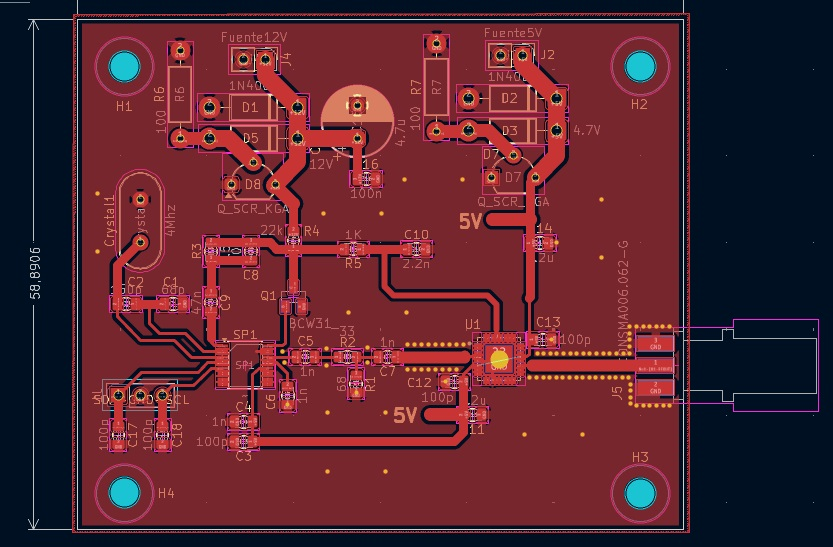
\includegraphics[width=0.85\textwidth]{img/PCBRediseñadaConNuevaHuella}
	}
	\caption{Layout de la PCB rediseñada. Usando la huella SSOP 16}
	\label{fig:bloques_original}
\end{figure}
	
	\subsection{Montaje e integración}
	
	\begin{itemize}[leftmargin=*]
		\item Soldadura de componentes SMD, incluyendo el VCO HMC534LP5 (QFN 5$\times$5\,mm) y el
		nuevo SP\,5769 con encapsulado adaptado.
		\item Programación inicial del ESP32 con el nuevo firmware.
		\item Integración mecánica: se diseñó y fabricó mediante \textbf{impresión 3D} un gabinete a medida
		para alojar el sistema completo y proteger las conexiones.
	\end{itemize}
	

	
	% ============================================================
	%  6. VALIDACIÓN
	% ============================================================
	\section{Validación funcional}
	
	\subsection{Metodología de medición}
	
	Las mediciones de validación se realizaron en el \textbf{banco de microondas} del Laboratorio de
	Telecomunicaciones de la FCEyT–UNT. Para determinar la frecuencia real emitida ($f_0$), se midió la
	longitud de onda dentro de la guía de onda ($\lambda_g$) utilizando el \textbf{ondámetro de ranura
		resonante}. Conociendo la dimensión transversal de la guía utilizada ($2a = 45{,}72$\,mm, que define
	la longitud de onda de corte $\lambda_c$), se calculó la longitud de onda en el espacio libre ($\lambda_0$)
	mediante la relación:
	
	\begin{equation}
		\frac{1}{\lambda_0^2} = \frac{1}{\lambda_g^2} + \frac{1}{\lambda_c^2}
		\label{eq:lambda}
	\end{equation}
	
	Finalmente, la frecuencia de oscilación se obtuvo como $f_0 = c / \lambda_0$, donde $c$ es la velocidad
	de la luz en el vacío.
	
	\subsection{Ensayos realizados}
	
	\subsubsection{Prueba de límites físicos del VCO (bomba de carga)}
	
	Para verificar la excursión máxima del VCO instalado, se forzaron por software los estados extremos
	de la bomba de carga del SP\,5769:
	
	\begin{itemize}[leftmargin=*]
		\item \textbf{CP-Disable (límite inferior):} Con la bomba de carga deshabilitada, la tensión de
		sintonía cae al mínimo. Se midió $\lambda_g = 42{,}52$\,mm, obteniendo una frecuencia límite
		inferior de $f_{min} \approx 9{,}3$\,GHz.
		\item \textbf{CP-Sink (límite superior):} Con la bomba de carga forzada a drenar corriente máxima,
		la tensión alcanza el límite superior. Se midió $\lambda_g = 29{,}12$\,mm, obteniendo una
		frecuencia límite superior de $f_{max} \approx 12{,}21$\,GHz.
	\end{itemize}
	
	Estos resultados confirman que el hardware supera holgadamente el rango requerido (10{,}6–11{,}8\,GHz).
	
	\subsubsection{Validación del enclavamiento de frecuencia}
	
	Se realizó un barrido discreto programando el sintetizador en saltos de 300\,MHz a lo largo de la banda
	de trabajo. La Tabla~\ref{tab:resultados} muestra los resultados comparativos entre la frecuencia
	programada ($f_{prog}$) y la frecuencia medida ($f_{med}$).
	
	\begin{table}[H]
		\centering
		\caption{Resultados de validación del enclavamiento PLL.}
		\label{tab:resultados}
		\renewcommand{\arraystretch}{1.3}
		\begin{tabular}{cccc}
			\toprule
			$f_{prog}$ (GHz) & $\lambda_g$ medida (mm) & $f_{med}$ (GHz) & Error relativo (\%) \\
			\midrule
			10{,}600 & 35{,}94 & 10{,}608 & 0{,}075 \\
			10{,}900 & 34{,}41 & 10{,}911 & 0{,}101 \\
			11{,}200 & 33{,}00 & 11{,}210 & 0{,}089 \\
			11{,}500 & 31{,}69 & 11{,}518 & 0{,}157 \\
			11{,}800 & 30{,}52 & 11{,}818 & 0{,}153 \\
			\bottomrule
		\end{tabular}
	\end{table}
	
	\subsubsection{Barrido de frecuencia (\textit{frequency sweep})}
	
	Se implementó y ensayó por software la función de barrido de frecuencia, verificando que el sistema
	puede recorrer toda la banda operativa de forma continua y estable.
	
	\subsection{Resultados}
	
	\begin{tcolorbox}[colback=grisClaro, colframe=azulUNT, title=\textbf{Síntesis de resultados}]
		\begin{itemize}[leftmargin=*]
			\item El PLL logró enclavamiento (\textit{lock}) en todos los puntos de frecuencia ensayados.
			\item El error relativo máximo observado fue del \textbf{0{,}157\%}, considerado despreciable para
			la aplicación educativa prevista.
			\item El VCO cubre con holgura el rango Ku requerido: desde 9{,}3\,GHz hasta 12{,}21\,GHz.
			\item El sistema operó de forma estable a lo largo de toda la banda 10{,}6–11{,}8\,GHz.
		\end{itemize}
	\end{tcolorbox}
	
	\subsection{Hardware principal y transmisión de la señal}
	
	El sistema se centra en la generación, transmisión y recepción de ondas electromagnéticas en el rango de las microondas (banda Ku). El núcleo de emisión es el sintetizador operando en un rango de 10{,}6\,GHz a 11{,}8\,GHz. Para acondicionar y caracterizar la señal, el banco cuenta con atenuadores de baja precisión (hasta 20\,dB) y de alta precisión (ajuste micrométrico de 0{,}01\,mm), además de un ondámetro de cavidad resonante.
	
	\begin{figure}[H]
		\centering
		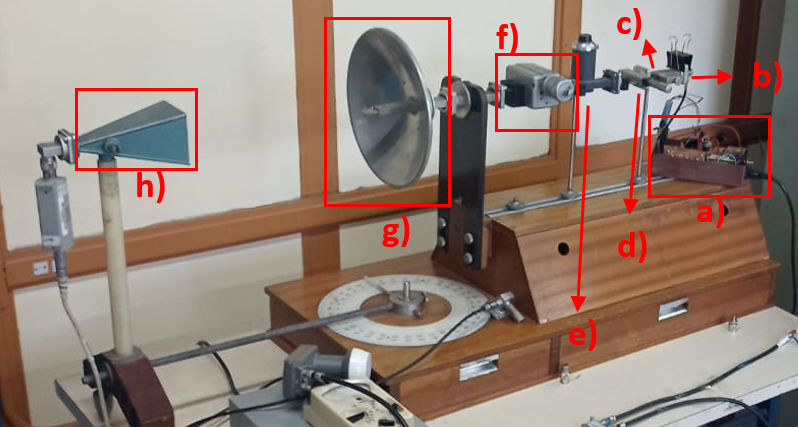
\includegraphics[width=0.7\textwidth]{images/image25.png}
		\caption{Configuración del banco de microondas.}
		\label{fig:banco_original}
	\end{figure}

	La onda viaja por la guía hasta la antena transmisora, la cual está conformada por un dipolo y un reflector parabólico que irradia con una polarización lineal vertical. En el extremo receptor, el campo es captado por una antena tipo bocina piramidal (\textit{Horn}). Para cuantificar la energía recibida, la antena se acopla a un diodo rápido Schottky montado en posición vertical, el cual rectifica la señal de RF para ser leída por un amperímetro analógico.

	\begin{figure}[H]
		\centering
		\begin{subfigure}{0.35\textwidth}
			\centering
			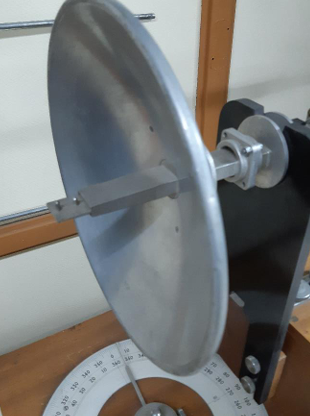
\includegraphics[height=5.5cm]{images/image27.png}
			\caption{Transmisor parabólico}
		\end{subfigure}
		\hfill
		\begin{subfigure}{0.35\textwidth}
			\centering
			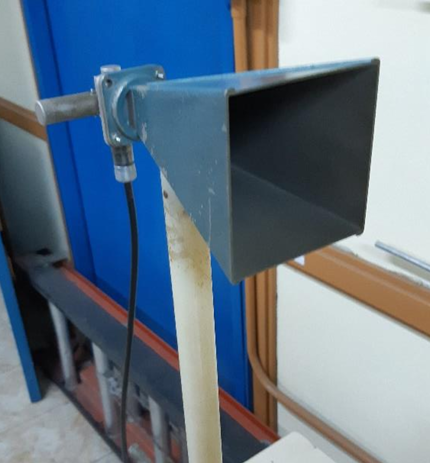
\includegraphics[height=5.5cm]{images/image37.png}
			\caption{Receptor de bocina}
		\end{subfigure}
		\caption{Antenas de transmisión y recepción en el banco.}
		\label{fig:antenas_banco}
	\end{figure}
	
	\subsection{Mediciones adicionales en banco con LNB}

	Como actividad extra, se integró en la recepción un LNB (\textit{Low Noise Block}) dual para bajar en frecuencia la señal de la banda Ku y permitir su análisis con un analizador de espectro de menor rango.
	Este dispositivo capta las frecuencias y las amplifica con bajo ruido, realizando una conversión a frecuencia intermedia (IF) mediante un oscilador local (OL).

	\begin{figure}[H]
		\centering
		\begin{subfigure}{0.65\textwidth}
			\centering
			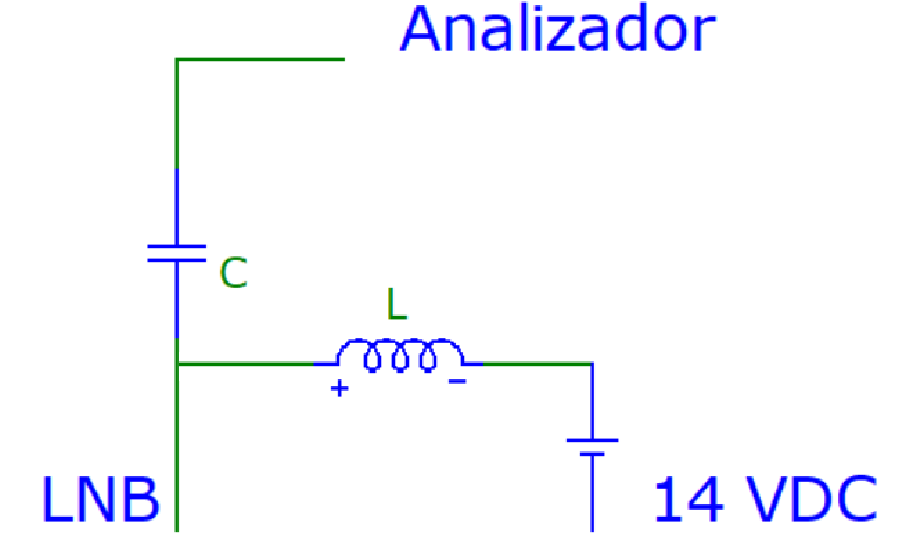
\includegraphics[width=0.9\linewidth]{images/image29.png}
			\caption{Conexión del LNB al montaje}
		\end{subfigure}
		\hfill
		\begin{subfigure}{0.3\textwidth}
			\centering
			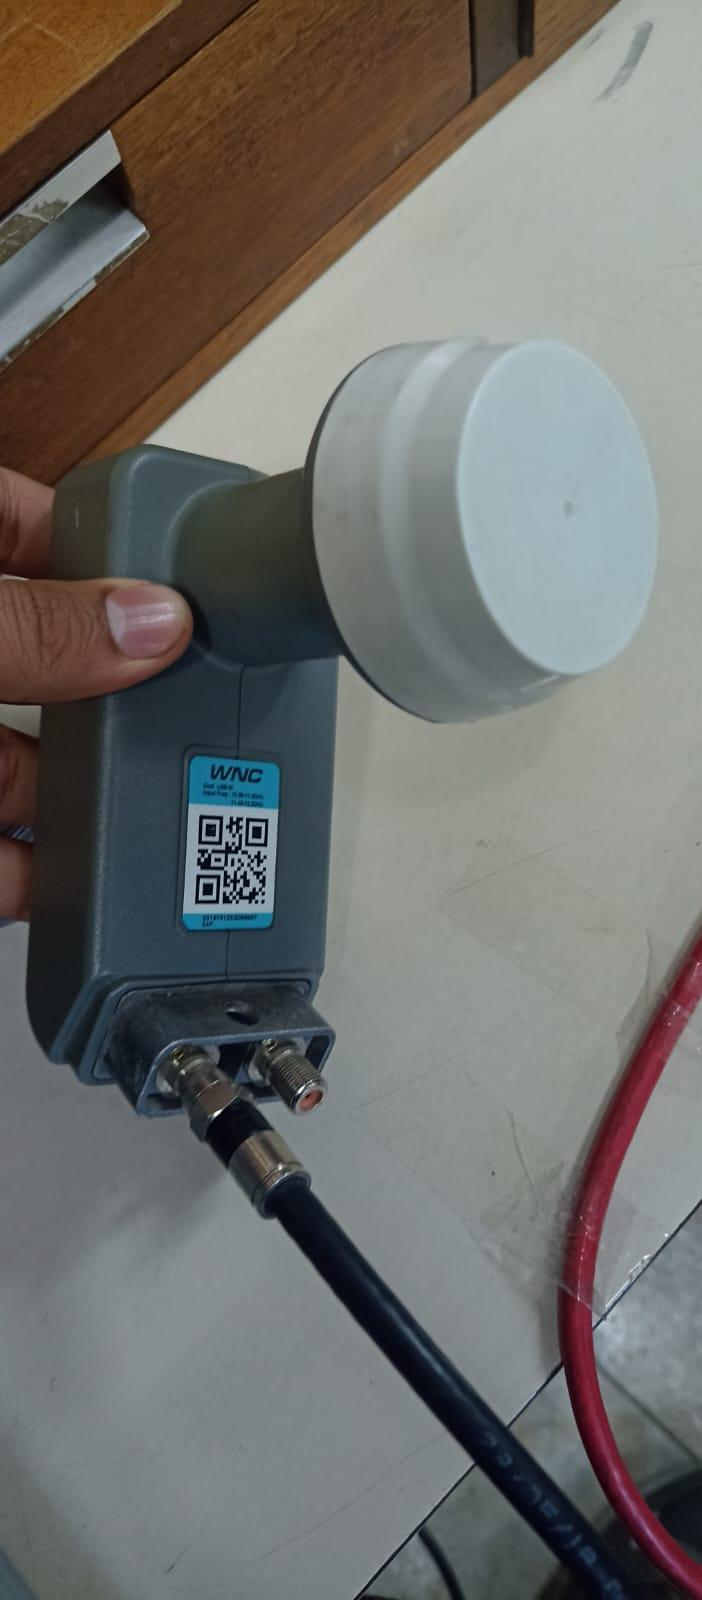
\includegraphics[width=0.9\linewidth]{images/image22.jpg}
			\caption{LNB dual}
		\end{subfigure}
		\caption{Integración de LNB en el banco experimental.}
		\label{fig:lnb}
	\end{figure}

	\paragraph{Inyector y filtro activo LC (Winegard PS-1403):}
	Para la correcta operación del LNB, se empleó un filtro inyector de continua (Winegard PS-1403) actuando como \textit{bias tee}. Esto permitió alimentar el LNB con continua sin afectar el paso de la señal de RF hacia el analizador de espectro, protegiendo sus puertos de entrada.

	\begin{figure}[H]
		\centering
		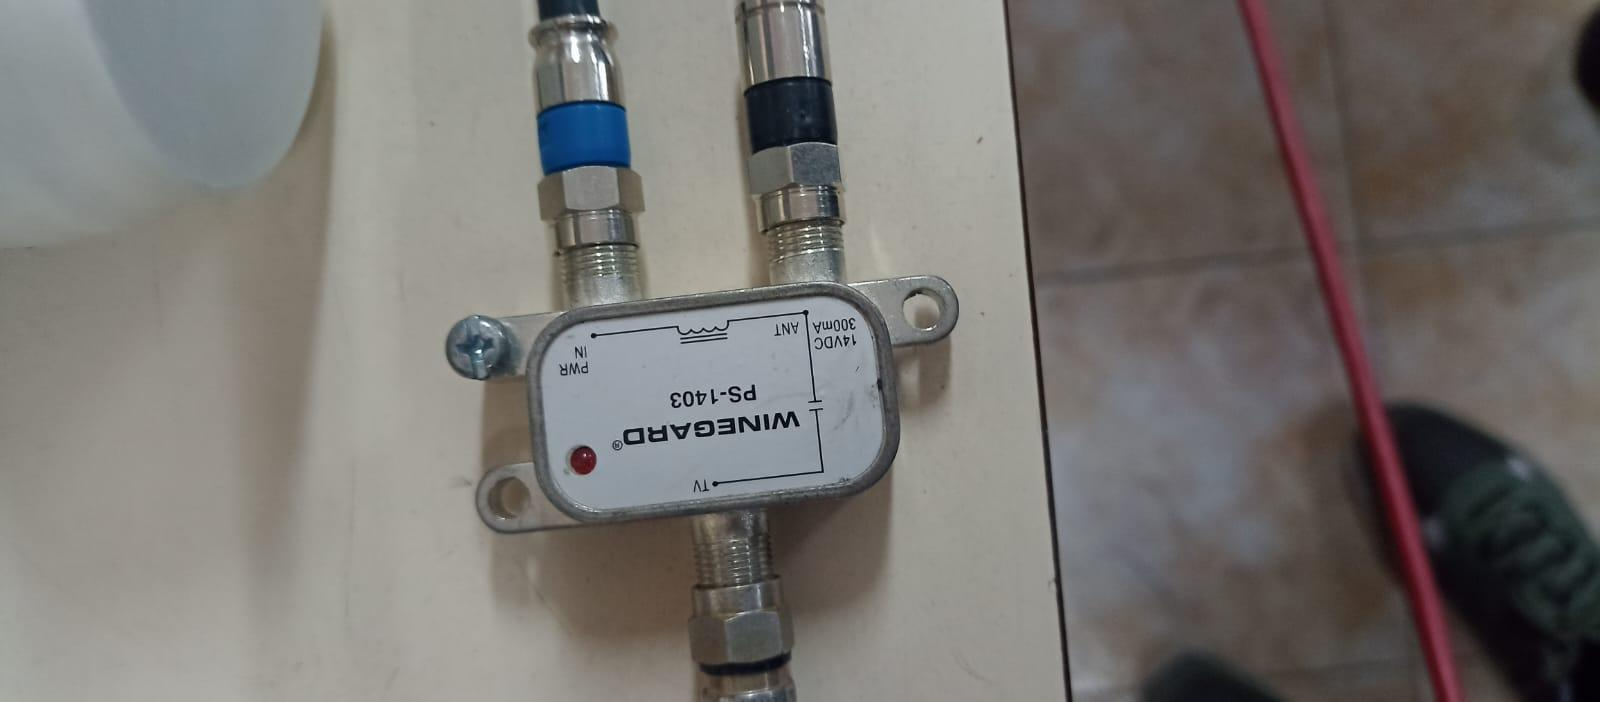
\includegraphics[width=0.7\textwidth]{images/image26.jpg}
		\caption{Filtro activo LC empleado para aislamiento y alimentación.}
		\label{fig:filtro_winegard}
	\end{figure}

	\begin{figure}[H]
		\centering
		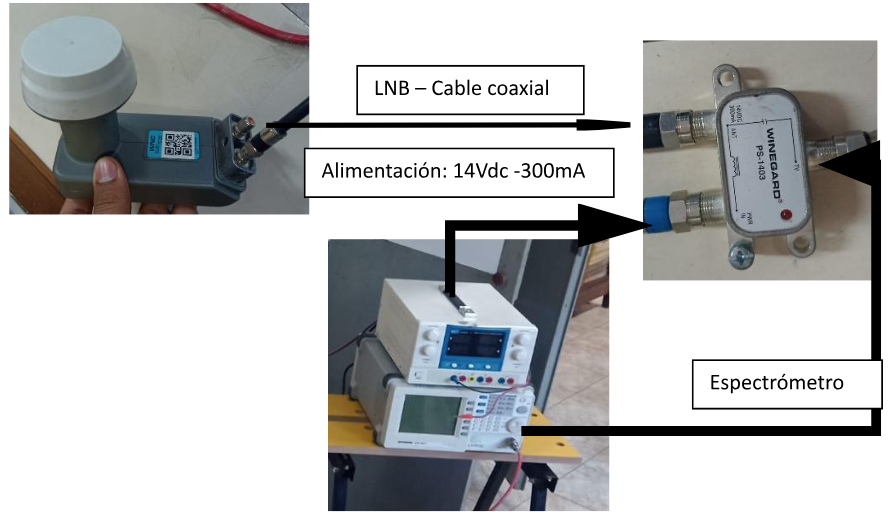
\includegraphics[width=0.6\textwidth]{images/image28.png}
		\caption{Esquema de conexiones con el analizador de espectro.}
		\label{fig:esquema_general}
	\end{figure}

	\paragraph{Lecturas de frecuencia convertida:}
	En el analizador de espectro se identificó correctamente el tono convertido a frecuencia intermedia $f_{IF} \approx 1{,}9$\,GHz.

	\begin{figure}[H]
		\centering
		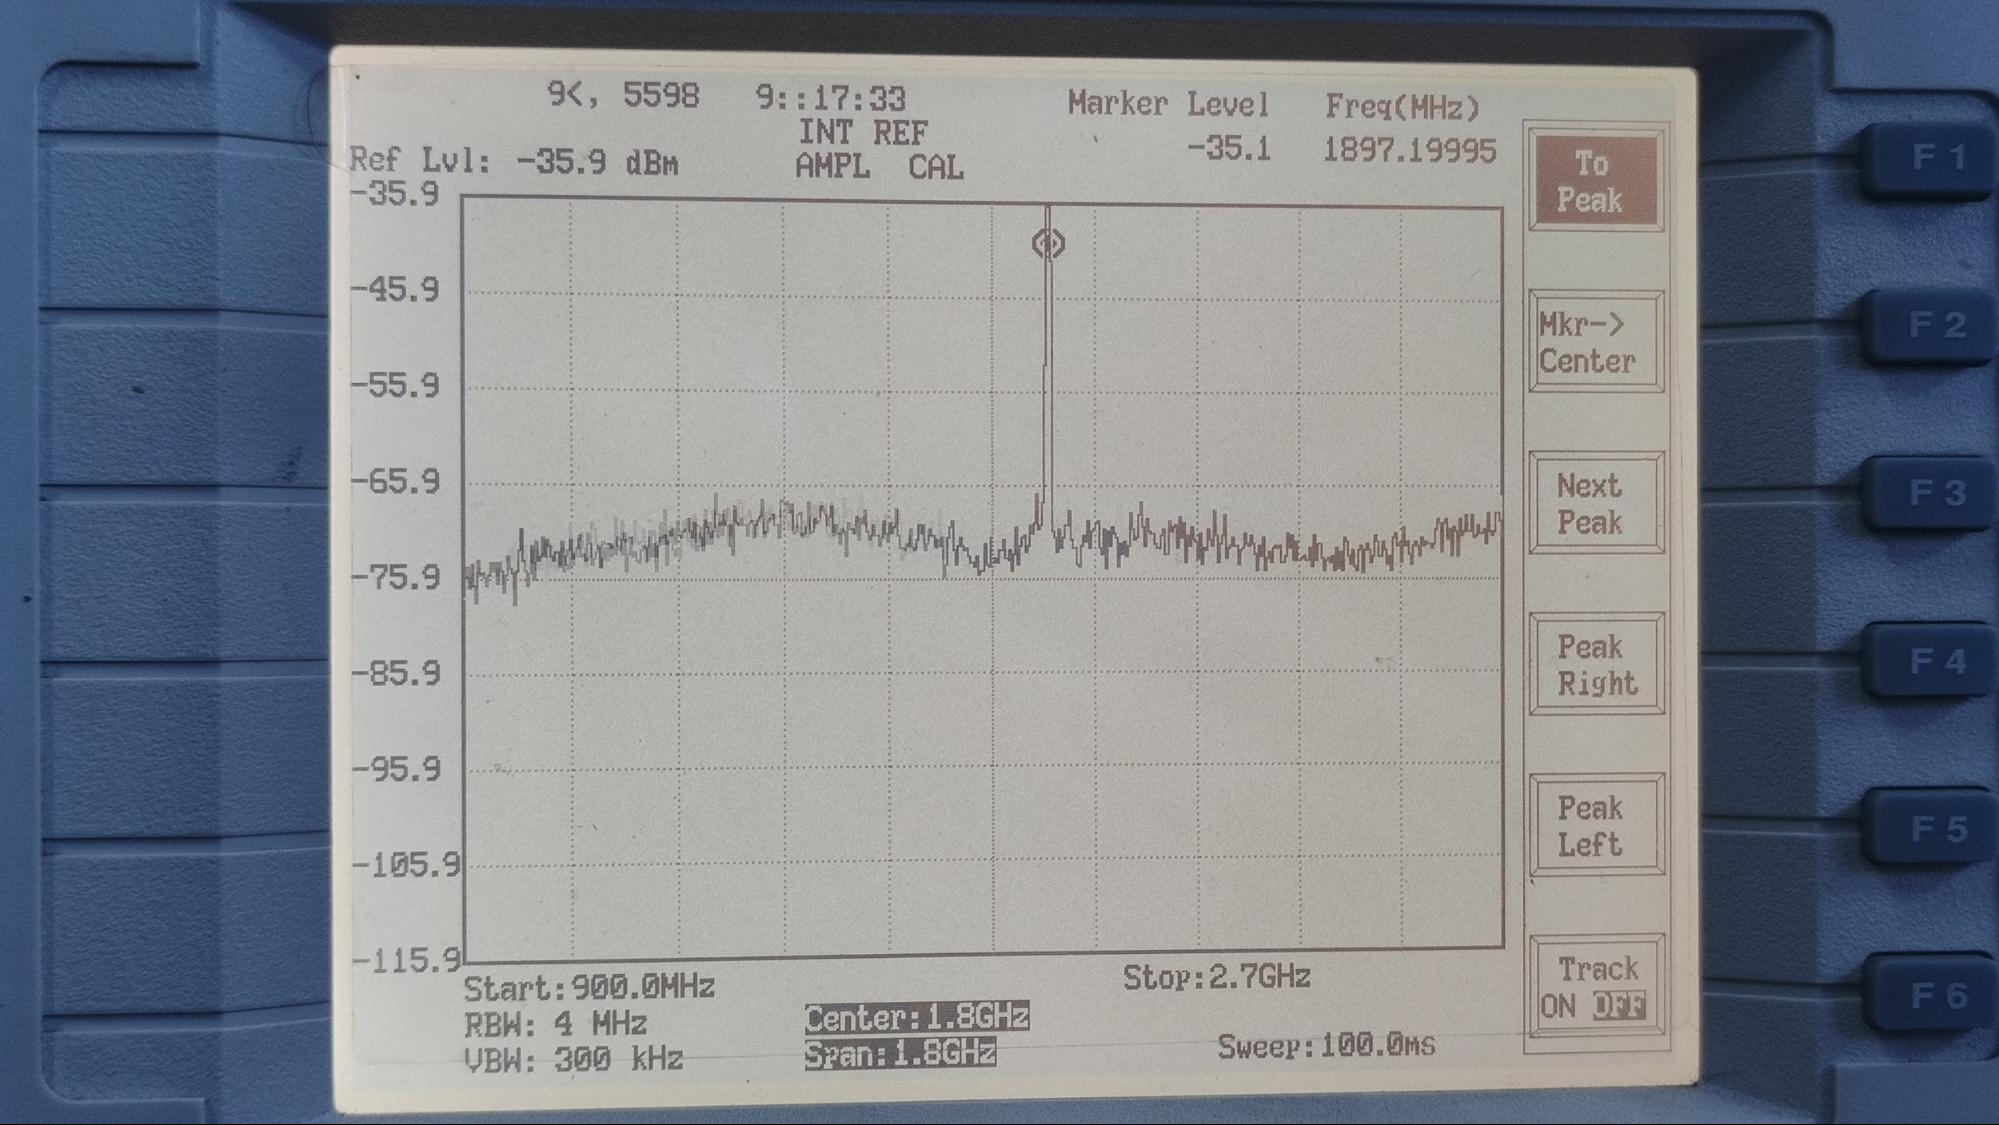
\includegraphics[width=0.6\textwidth]{images/image33.jpg}
		\caption{Tono medido en el analizador de espectro.}
		\label{fig:medicion_espectro}
	\end{figure}

	Sabiendo la frecuencia transmitida por el oscilador ($f_{RF}$) y la frecuencia detectada en el analizador ($f_{IF}$), se verifica empíricamente la frecuencia del oscilador local ($f_{OL}$) interno del LNB utilizando la relación fundamental de los mezcladores:
	\begin{equation}
		f_{OL} = f_{RF} - f_{IF} = 11{,}65\,\text{GHz} - 1{,}90\,\text{GHz} = 9{,}75\,\text{GHz}
	\end{equation}

	% ============================================================
	%  7. RESULTADOS Y CONCLUSIONES
	% ============================================================
	\section{Resultados y conclusiones}
	
	\subsection{Logros obtenidos}
	
	Se logró recuperar la funcionalidad completa del sintetizador de frecuencias en banda Ku. El sistema
	final opera correctamente en el rango 10{,}6–11{,}8\,GHz con un error de frecuencia inferior al
	0{,}16\%, confirmado mediante mediciones en banco de microondas.
	
	El rediseño integral de la PCB permitió:
	
	\begin{itemize}[leftmargin=*]
		\item Adaptar el diseño a los encapsulados de componentes actualmente disponibles en el mercado.
		\item Resolver los problemas de integridad de señal presentes en la placa heredada.
		\item Garantizar la reproducibilidad y el mantenimiento del equipo para uso educativo a largo plazo.
		\item Mejorar sustancialmente la interfaz de usuario mediante la incorporación de comunicación
		Bluetooth y una pantalla de visualización.
	\end{itemize}
	
	\subsection{Lecciones aprendidas}
	
	\begin{itemize}[leftmargin=*]
		\item La importancia del diseño de PCB orientado a la integridad de señal en alta frecuencia desde
		la etapa de concepción, para evitar problemas de reparabilidad en el futuro.
		\item La necesidad de documentar todos los intentos de reparación sobre hardware heredado para
		facilitar el diagnóstico posterior.
		\item El valor de contar con equipamiento especializado (estación de soldadura para QFN, banco de
		microondas) para proyectos de RF en banda Ku.
	\end{itemize}
	

	
	% ============================================================
	%  REFERENCIAS
	% ============================================================
	
	
	% ============================================================
	%  ANEXOS
	% ============================================================
	\newpage
	\appendix
	
	\section{Informe de actividades de laboratorio (29/08/2024)}
	\label{anx:informe_lab}
	
	
	\bigskip
	\noindent\rule{\textwidth}{0.4pt}
	
	\textbf{Fecha:} 29 de agosto de 2024\\
	\textbf{Responsable:} Jesús Avila\\
	\textbf{Proyecto:} Reparación de Sintetizador de Frecuencias\\
	\textbf{Ubicación:} Laboratorio de Telecomunicaciones
	
	\paragraph{Descripción del trabajo realizado.}
	Se realizaron tareas de diagnóstico y reparación en un sintetizador compuesto por un módulo de RF
	con sintetizador SP\,5769, VCO y placa ESP32 (interfaz Bluetooth). El firmware de la ESP32 había
	sido validado previamente (lógica mediante TDD y comunicación I2C con una BluePill programada con
	la dirección del SP\,5769).
	
	\paragraph{Procedimiento.}
	\begin{enumerate}[leftmargin=*, label=\textbf{\arabic*.}]
		\item \textbf{Conexión inicial:} Se conectó la ESP32 al módulo de RF a través del conector DB9.
		\item \textbf{Verificación de conexiones:} Con multímetro se detectó y corrigió un error en la
		referencia de conexiones.
		\item \textbf{Prueba de comunicación:} Usando la aplicación \textit{Bluetooth Terminal}, se confirmó
		que el SP\,5769 respondía correctamente, aunque no lograba el enclavamiento.
		\item \textbf{Verificación de potencia de salida:} Tanto con sensor rectificador/medidor analógico
		como con analizador de RF digital, se constató ausencia total de potencia de salida.
	\end{enumerate}
	
	\paragraph{Resultados y conclusiones.}
	La ausencia de potencia de salida y la falta de enclavamiento indicaron falla en el VCO o en el
	transistor externo. Se propuso un análisis más profundo de ambos componentes para confirmar la causa.
	
	\noindent\rule{\textwidth}{0.4pt}
-----------------------------
	\section{Configuración de registros del SP\,5769}
	\label{anx:registros}
	
\begin{table}[H]
	\centering
	\caption{Bytes en modo lectura del SP5769.}
	\label{tab:sp5769_lectura}
	\renewcommand{\arraystretch}{1.3}
	\begin{tabular}{llccccccccc}
		\toprule
		& & \multicolumn{8}{c}{\textbf{MSB $\longleftarrow$ \hspace{3cm} $\longrightarrow$ LSB}} & \\
		\midrule
		\textbf{Byte 1} & Dirección & 1 & 1 & 0 & 0 & 0 & 1 & 0 & A \\
		\textbf{Byte 2} & Status    & POR & FL & 0 & 0 & 0 & 0 & 0 & A \\
		\bottomrule
	\end{tabular}
\end{table}

\begin{table}[H]
	\centering
	\caption{Bytes de configuración de escritura SP5769.}
	\label{tab:sp5769_escritura}
	\renewcommand{\arraystretch}{1.3}
	\begin{tabular}{llccccccccc}
		\toprule
		& & \multicolumn{8}{c}{\textbf{MSB $\longleftarrow$ \hspace{3cm} $\longrightarrow$ LSB}} & \\
		\midrule
		\textbf{Byte 1} & Dirección      & 1 & 1 & 0 & 0 & 0 & 1 & 0 & A \\
		\textbf{Byte 2} & Divisor prog.\ 0 & $2^{14}$ & $2^{13}$ & $2^{12}$ & $2^{11}$ & $2^{10}$ & $2^{9}$ & $2^{8}$ & A \\
		\textbf{Byte 3} & Divisor prog.\ 2 & 2 & 2 & 2 & 2 & 2 & 2 & 2 & A \\
		\textbf{Byte 4} & Control        & 1 & 0 & 0 & 0 & R3 & R2 & R1 & R0 & A \\
		\textbf{Byte 5} & Control        & 0 & 0 & 0 & 0 & 0 & 0 & 0 & 0 & A \\
		\bottomrule
	\end{tabular}
\end{table}

\begin{table}[H]
	\centering
	\caption{Configuración del divisor de referencia (bits R3--R0).}
	\label{tab:divisor_referencia}
	\renewcommand{\arraystretch}{1.25}
	\begin{tabular}{cccc>{\bfseries}c}
		\toprule
		\textbf{R3} & \textbf{R2} & \textbf{R1} & \textbf{R0} & Divisor de referencia \\
		\midrule
		0 & 0 & 0 & 0 & 2   \\
		0 & 0 & 0 & 1 & 4   \\
		0 & 0 & 1 & 0 & 8   \\
		0 & 0 & 1 & 1 & 16  \\
		0 & 1 & 0 & 0 & 32  \\
		0 & 1 & 0 & 1 & 64  \\
		0 & 1 & 1 & 0 & 128 \\
		0 & 1 & 1 & 1 & 256 \\
		1 & 0 & 0 & 0 & 24  \\
		1 & 0 & 0 & 1 & 5   \\
		1 & 0 & 1 & 0 & 10  \\
		1 & 0 & 1 & 1 & 20  \\
		1 & 1 & 0 & 0 & 40  \\
		1 & 1 & 0 & 1 & 80  \\
		1 & 1 & 1 & 0 & 160 \\
		1 & 1 & 1 & 1 & 320 \\
		\bottomrule
	\end{tabular}
\end{table}
	% -------------------------------------------------------

	% -------------------------------------------------------
 -------------------------------------------------------
	\section{Mediciones adicionales}
	\label{anx:mediciones}
	
\begin{figure}[H]
	\centering
	\fcolorbox{azulUNT}{white}{
		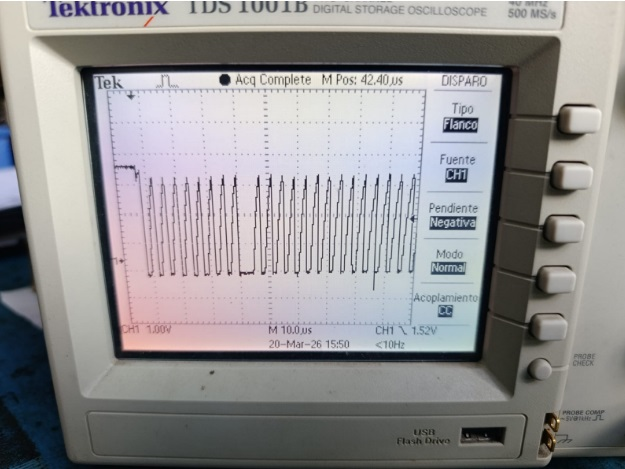
\includegraphics[width=0.85\textwidth]{img/I2CmsgSCL}
	}
	\caption{Mensaje I2C, pin SCL}
	\label{fig:i2cmsgscl}
\end{figure}


\begin{figure}[H]
	\centering
	\fcolorbox{azulUNT}{white}{
		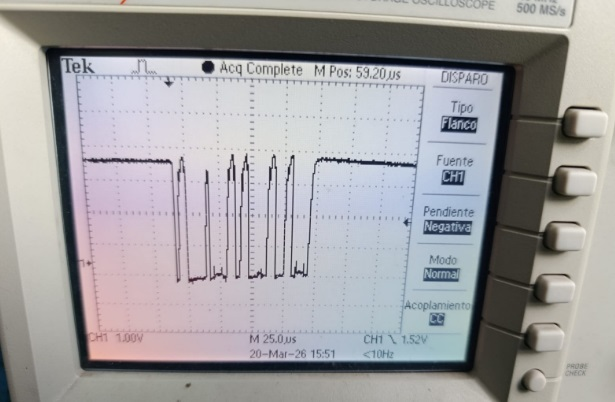
\includegraphics[width=0.85\textwidth]{img/I2CmsgSDA}
	}
	\caption{Mensaje I2C, pin SDS}
	\label{fig:i2cmsgsda}
\end{figure}	

\begin{figure}[H]
	\centering
	\fcolorbox{azulUNT}{white}{
		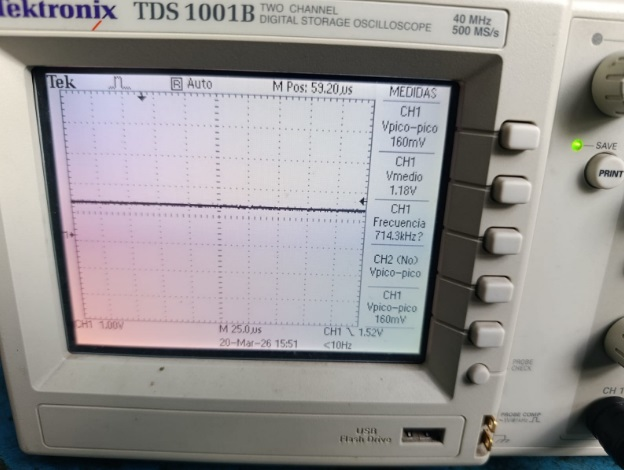
\includegraphics[width=0.85\textwidth]{img/ADRESSvalue}
	}
	\caption{Medicion del pin ADRESS, el cual determina la dirección del dispositivo}
	\label{fig:addrs}
\end{figure}	

\begin{figure}[H]
	\centering
	\fcolorbox{azulUNT}{white}{
		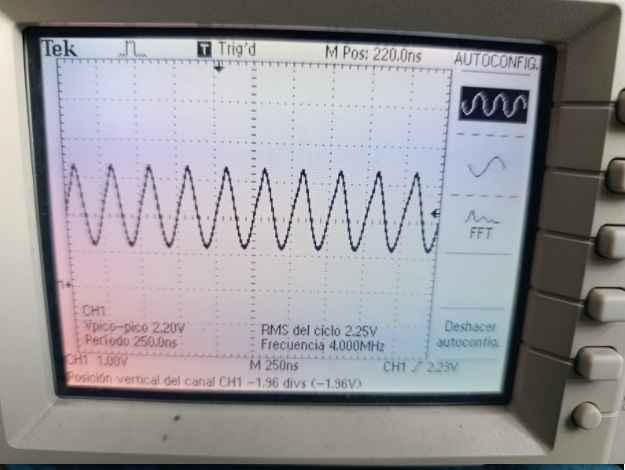
\includegraphics[width=0.85\textwidth]{img/xtalOsc}
	}
	\caption{Señal de 4 Mhz en el cristal}
	\label{fig:4mhzosc}
\end{figure}	

\newpage
\section*{Referencias}
\addcontentsline{toc}{section}{Referencias}

\begin{enumerate}[leftmargin=*, label={[\arabic*]}]
	\item Phillips Semiconductors, \textit{SP5769 PLL Frequency Synthesizer Datasheet}. 
	\item Analog Devices (Hittite), \textit{HMC534LP5 VCO Datasheet}. 
	\item Espressif Systems, \textit{ESP32 Technical Reference Manual}. Disponible en: \url{https://www.espressif.com/}
\end{enumerate}
\end{document}